\chapter{Proposed improvements and results}
\label{cha:improvements}

In this chapter, we will present some improvements to live streaming protocols and libraries that we believe produce a better overall quality of experience in video streaming. The proposed improvements are based on the findings presented in the previous chapter.

Specifically, we will first dive into the adaptation algorithms of DASH.js to assess that the default configuration is not suitable for low-latency live streaming. Then, we will propose a better configuration which also involves writing a custom ABR rule.

We will then look at how we can play with HTTP/3 priorities to give priority to audio segments. We will implement this part with hls.js. To overcome the fact that Chromium's buffer underflow behavior (Section \ref{sec:eval/non-abr/http-versions}) is limited to 3 seconds and that it is not available on other browsers, we will use the \texttt{WebCodecs} API to implement the generation of a "filler" segment for when no video segment is available. This also allows to cancel the loading of the segment when it is too late for it to arrive, therefore saving bandwidth.

Finally, we will show how this solution produces fewer playback stalls and what possible improvements are left for future work.

\section{DASH.js bitrate adaptation algorithm improvements}
\label{sec:improvements/dashjs}

In Section \ref{sec:eval/abr/dashjs} we have shown how in some cases the default configuration of DASH.js makes the video quality oscillate too frequently with a live stream with low latency. Specifically, Figure \ref{fig:eval_abr_dashjs} represents the buffer health plot, where we can see that in the second half of the experiment the media bitrate chosen by DASH.js frequently changes and most of the time stays at a lower value than it should, even if the network bandwidth is consistently above 8 Mbps.

The decision on which bitrate should be requested next is the task of the rate adaptation algorithm, which every library typically implements differently. There are in fact many approaches to solving the problem and there is no clear consensus on which is the best.

The core idea of adaptation algorithms is to choose the best quality level so that the bitrate is lower than the available network bandwidth. There are two main approaches to making this decision:

\begin{itemize}
    \item \textbf{Throughput-based}: the most intuitive approach, consisting of continuously calculating an estimate of the network bandwidth and then selecting the highest bitrate in the ladder which is lower than the bandwidth estimate.
    \item \textbf{Buffer-based}: an alternative approach that observes the occupancy of the buffer to determine whether the decision to increase/dicrease the bitrate should be made. This approach avoids the need to keep a bandwidth estimate.
\end{itemize}

DASH.js uses a combination of these two approaches with a strategy called \texttt{DYNAMIC}, first presented in \cite{dashjs_dynamic}. The \texttt{DYNAMIC} strategy switches between a throughput-based approach, named \texttt{THROUGHPUT}, and a buffer-based approach, \texttt{BOLA}.\cite{bola} The idea of switching between the two is based on the fact that each algorithm works best in different situations. In particular, the throughput-based algorithm performs better when the buffer is low or empty, while \texttt{BOLA} (buffer-based) performs better when the buffer level is sufficiently large.

The algorithm that switches between \texttt{THROUGHPUT} and \texttt{BOLA} is therefore based on a threshold that is applied on the buffer level (for each media track). The following code snippet taken from the DASH.js source code (\texttt{AbrController} class) shows how the decision on whether to use \texttt{BOLA} is implemented:

\begin{minted}[frame=single,linenos,breaklines,highlightlines=2]{js}
const useBufferABR = isUsingBufferOccupancyAbrDict[mediaType];
const newUseBufferABR = bufferLevel > (useBufferABR ? switchOffThreshold : switchOnThreshold);
isUsingBufferOccupancyAbrDict[mediaType] = newUseBufferABR;

if (newUseBufferABR !== useBufferABR) {
    if (newUseBufferABR) {
        logger.info('[' + mediaType + '] switching from throughput to buffer occupancy ABR rule');
    } else {
        logger.info('[' + mediaType + '] switching from buffer occupancy to throughput ABR rule');
    }
}
\end{minted}

The relevant line is line 2, where the new decision on whether buffer-based ABR should be used is made based on whether the current buffer level (in seconds) is greater than a threshold.

The \texttt{switchOffThreshold}/\texttt{switchOnThreshold} is calculated from the value of a property called \texttt{stableBufferTime}. Basically, when the buffer level exceeds a threshold value that is considered stable, the \texttt{DYNAMIC} algorithm switches to the buffer-based approach (\texttt{BOLA}), while going back to \texttt{THROUGHPUT} when the buffer level is less than half of the \texttt{stableBufferTime}.

\begin{minted}[frame=single]{js}
const switchOnThreshold = stableBufferTime;
const switchOffThreshold = 0.5 * stableBufferTime;
\end{minted}

The aim is to avoid continuous oscillations between the two strategies, although this does not work well in practice according to our tests. In fact, in the case of a live stream, \texttt{stableBufferTime} is assigned to the live delay target (a configuration parameter, see Section \ref{sec:testbed/frontend/dashjs}). So, for example, if the live delay is 4 seconds, this means that the \texttt{DYNAMIC} algorithm will switch from \texttt{THROUGHPUT} to \texttt{BOLA} when the buffer level goes above 4 seconds, and will switch back to \texttt{THROUGHPUT} when the buffer level goes below 2 seconds.

The problem is that with such a low target live latency, the buffer level tends to oscillate quite a lot and often goes below the threshold of 2 seconds, as can be seen in Figure \ref{fig:eval_abr_dashjs}, for example. In practice, this means that the default \texttt{DYNAMIC} ABR strategy of DASH.js will switch between the two approaches very often. This behavior is probably undesirable, as it does not leave time for the algorithm to make proper decisions.

This behavior is also in contrast to the threshold used by the paper that introduced \texttt{DYNAMIC} and tested its performance. In fact, in \cite{dashjs_dynamic} the threshold value is fixed at 10 seconds. Therefore, following the recommendation in \cite{dashjs_dynamic} we decided to disable the \texttt{DYNAMIC} strategy and force the \texttt{THROUGHPUT} one. This can be done in DASH.js through settings:

\begin{minted}[frame=single]{js}
player.updateSettings({
    streaming: {
        abr: {
            ABRStrategy: 'abrThroughput'
        }
    }
});
\end{minted}

While we were looking at the internals of DASH.js to investigate the issue with \texttt{DYNAMIC}, we discovered that the library includes support for \textbf{additional ABR rules} that should help in cases when the ABR strategy is not enough to make proper decisions about the next bitrate. These rules are by default:

\begin{itemize}
    \item \texttt{DroppedFramesRule}: measures the dropped frames during playback. If they exceed 15\%, the ruel switches to a lower bitrate.
    \item \texttt{SwitchHistoryRule}: observes the switch history and avoids switches to higher bitrates that caused quality drops in the past, according to the switch history.
    \item \texttt{AbandonRequestsRule}: calculates whether the loading of a segment should be canceled because it is estimated that it will not be loaded in time for playback, only if there is a lower bitrate that could instead be loaded in the remaining time. This rule acts as an emergency switch down.
    \item \texttt{InsufficientBufferRule}: this rule puts an upper limit on the bitrate, depending on the current buffer health.
\end{itemize}

In particular, the \texttt{InsufficientBufferRule} was found to be the most aggressive in lowering the bitrate even when it was not needed. This happens because it bases the decision on the buffer level, which, as we have seen, is always quite small in a low-latency scenario. More in detail, the \texttt{InsufficientBufferRule} listens to the \texttt{BUFFER\_EMPTY} event and requests the switch to the minimum bitrate when that happens. Otherwise, the rule calculates the maximum bitrate to use as the limit depending on the throughput, so that a whole segment can be downloaded before the buffer runs out. The relevant lines of the rule that perform this computation are:

\begin{minted}[frame=single,linenos,breaklines,highlightlines=4]{js}
const throughput = throughputHistory.getAverageThroughput(mediaType, isDynamic);
const bufferLevel = dashMetrics.getCurrentBufferLevel(mediaType);
const fragmentDuration = representationInfo.fragmentDuration;
const bitrate = throughput * (bufferLevel / fragmentDuration) * INSUFFICIENT_BUFFER_SAFETY_FACTOR;
\end{minted}

Line 4 is where the upper limit is calculated. Since \texttt{(bufferLevel / fragmentDuration)} can be seen as the number/fraction of segments currently in the buffer, the maximum bitrate is calculated as a multiplication between the current throughput estimate and the number of segments in the buffer. However, there is a safety factor of 0.5 that effectively halves the maximum bitrate. When the bandwidth estimate is conservative (or still has to adapt to the new network conditions) or the buffer level is kept low on purpose to achieve lower latency, this rule tends to limit the video bitrate unnecessarily.

For these reasons, we decided to disable the \texttt{InsufficientBufferRule} and instead create a \textbf{custom rule} that acts only when the buffer is actually empty. In this way, we avoid overreactions of the algorithm deriving from the low latency. The rule can be disabled as follows:

\begin{minted}[frame=single]{js}
player.updateSettings({
    streaming: {
        abr: {
            ABRStrategy: 'abrThroughput'
            additionalAbrRules: {
                insufficientBufferRule: false
            }
        }
    }
});
\end{minted}

The new custom rule can instead be added using the method shown in the following code snippet, without having to modify and rebuild the library.

\begin{minted}[frame=single]{js}
player.addABRCustomRule('qualitySwitchRules', 'BufferEmptyRule', BufferEmptyRule);
\end{minted}

The implementation of the new \texttt{BufferEmptyRule} is similar to the original, but removes the maximum bitrate cap. Instead, it only forces a switch to the minimum bitrate when the buffer is empty. The following (simplified) code block shows how the check is performed.

\begin{minted}[frame=single,breaklines]{js}
if (currentBufferState.state === MetricsConstants.BUFFER_EMPTY) {
    logger.warning('[' + mediaType + '] BufferEmptyRule: switch to index 0.');
    switchRequest.quality = 0;
    switchRequest.reason = 'BufferEmptyRule: Buffer is empty';
}
\end{minted}

This tweaked configuration, consisting in forcing the \texttt{THROUGHPUT} strategy and modifying the additional rules, produces different results compared to previous experiments. For example, the experiment with the \texttt{lte} dataset no longer shows the issue of oscillating bitrate, as shown in Figure \ref{fig:improvements_dashjs}.

\begin{figure}
    \centering
    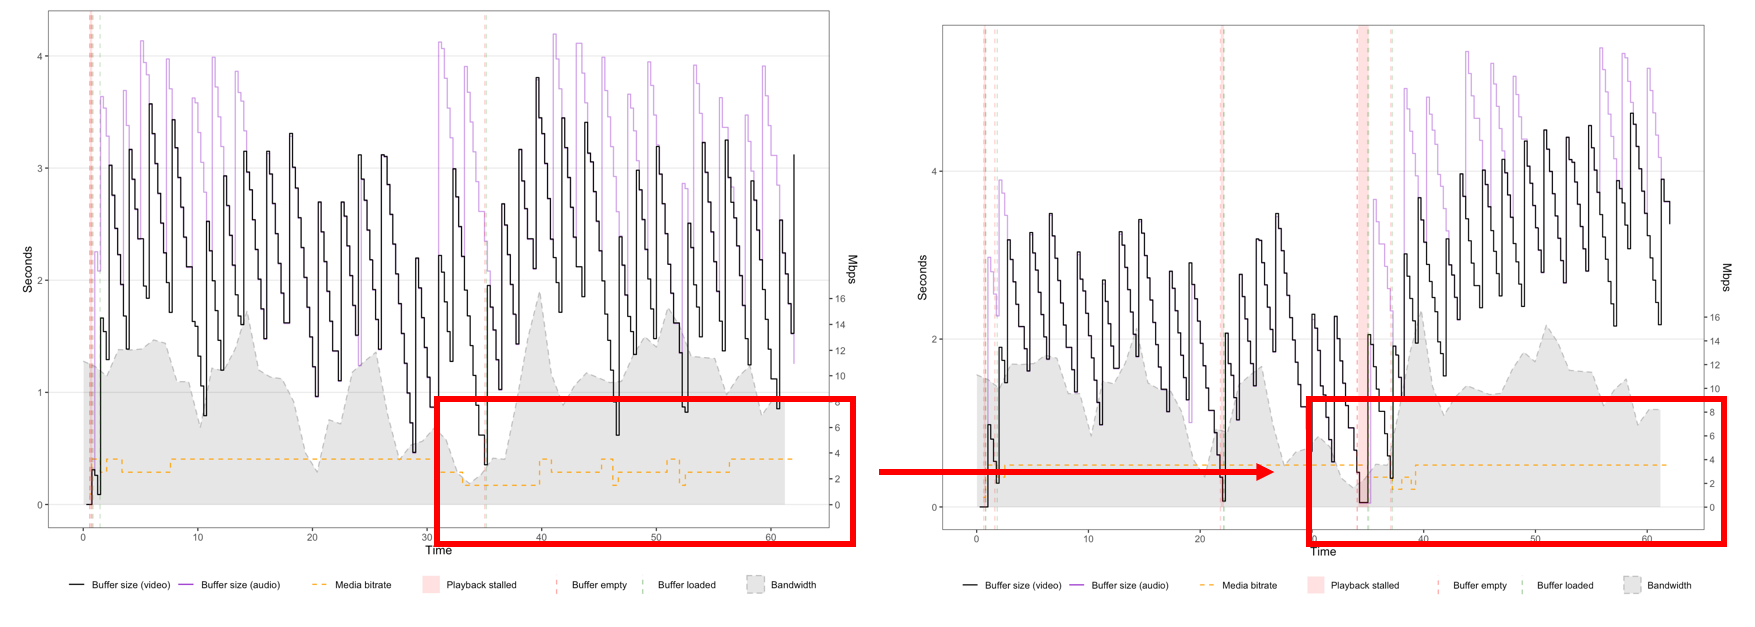
\includegraphics[width=\textwidth]{res/impr_dashjs.png}
    \caption{Buffer health plots showing the difference between the default DASH.js ABR configuration and the tweaked configuration.}
    \label{fig:improvements_dashjs}
\end{figure}

\section{Switching to hls.js}
\label{sec:improvements/hlsjs}

During the development of these improvements to DASH.js, we had the opportunity to take a deeper look at the internals and architecture of DASH.js. Unfortunately, we have found that most parts of the code are poorly documented and sometimes even have incomplete TypeScript types definitions. Also, our impression was that it was harder to understand how to extend the library and add new components. One of the reasons is that the library is using plain JavaScript, making it harder to have proper IDE support and type safety.

This led us to switch to hls.js for the rest of our work. Unlike DASH.js, hls.js is written in TypeScript and seems to be better documented. For example, the general architecture and design of the library is explained in detail in the official documentation.\footnote{\url{https://github.com/video-dev/hls.js/blob/master/docs/design.md}}

Unlike DASH.js, hls.js does not use a hybrid approach for the adaptation algorithm. Instead, it uses a standard \textbf{Exponential Weighted Moving Average} (EWMA) bandwidth estimator, which tracks bandwidth samples to produce an estimate of the available network bandwidth. This approach is used for both on-demand and live content, although with different configuration parameters for the EWMA computation.

In addition to the bandwidth estimate, hls.js also has an \textbf{abandon rule} similar to the one of DASH.js. This rule is implemented in the \texttt{\_abandonRulesCheck} method of the \texttt{AbrController} class and is periodically called by a timer. The method calculates the download rate of the current segment and estimates whether the segment will be loaded quickly enough to prevent buffer underflow, based on the estimate of bandwidth. If necessary, the rule will then find a quality level whose bitrate allows the segment to be loaded before buffer starvation, with a safety factor of 80\%. If no level matches this condition, the lower bitrate is chosen.

\section{Adding priority}
\label{sec:improvements/priority}

As we have seen in Section \ref{sec:eval/abr/hls}, using HLS with the \texttt{spike} pattern tends to produce playback stalls when the bandwidth abruptly drops. This was evident in Figure \ref{fig:eval_abr_hls}. In this section, we will look at how adding priority to some requests resolves this issue.

The easiest way to manipulate how hls.js sends HTTP requests is to use the \texttt{xhrSetup} or \texttt{fetchSetup} configuration options. They can be used to manipulate how HTTP requests are sent respectively with \texttt{XMLHttpRequest} or the \texttt{fetch} API, depending on how hls.js is configured. In our case we use the default XHR loader, so we would need to use the \texttt{xhrSetup} configuration option.

The \texttt{xhrSetup} option takes a function that is called just before sending the HTTP request. In practice, it allows to override how the request is created. In our case, to set the HTTP/3 priority we need to set either the \texttt{Priority} header or the \texttt{priority} query string parameter. In fact, in Section \ref{sec:eval/browsers/priorities} we introduced a patch to the \texttt{h2o} web server that lets us set the priority with the query string parameter.

Since we are interested in giving priority only to the audio segments requests, we need to distinguish which requests correspond to those segments. Doing so in the \texttt{xhrSetup} function does not give a proper way to distinguish the type of request so we must resort to looking at the format of the URL. Since the chunk files contain the ID of the stream (i.e. audio or video), we can implement priority for audio segment as follows.

\begin{minted}[frame=single]{ts}
const hls = new Hls({
    xhrSetup: (xhr, url) => {
        if (url.includes('chunk-stream-0')) {
            url = url + '?priority=1';
        } else {
            url = url + '?priority=2';
        }
        xhr.open('GET', url, true);
    }
});
\end{minted}

In this case, we are giving the chunks for stream 1 an HTTP/3 priority of \texttt{1}, while all the other files have priority \texttt{2} (still higher than the default of \texttt{3}).

A better way would be to override the \texttt{Hls} loader to override the URL of the segment based on its type. This is slightly more complex to implement, but we can still avoid to reimplement the whole loader implementation, taking advantage of inheritance.

\begin{minted}[frame=single,breaklines,highlightlines=6]{js}
class CustomLoader extends Hls.DefaultConfig.loader {
    constructor(config: HlsConfig) {
        super(config);
        const load = this.load.bind(this);
        this.load = (context: FragmentLoaderContext, config: LoaderConfiguration, callbacks: LoaderCallbacks<LoaderContext>) => {
            if (context.frag.type === 'audio') {
                context.url += '?priority=1';
            } else {
                context.url += '?priority=2';
            }
            load(context, config, callbacks);
        }
    }
}
\end{minted}

The custom fragment loader (\texttt{fLoader}) can then be passed as an option when creating the \texttt{Hls} instance:

\begin{minted}[frame=single]{ts}
const hls = new Hls({
    fLoader: CustomLoader as FragmentLoaderConstructor,
});
\end{minted}

After testing this configuration that gives priority to audio, we quickly discovered that the results were not what we expected. In particular, there were still playback stalls, and in some cases the audio buffer became empty. However, this should not happen since there is always enough bandwidth to transfer the audio segments, which are very small and require just a few hundreds of kbps to be downloaded.

Looking at the logs of hls.js (debug mode), we quickly found that the audio media playlist took several seconds to load. Without an updated playlist, HLS does not know which segment should be requested next. This is different from DASH, where \texttt{SegmentTemplate} allows the client to generate the URL of the segment without having to request the playlist again (Section \ref{sec:bg/technologies/dash}).

Consequently, if we want to give priority to audio, we need to also give priority to the corresponding media playlist, in addition to the segments. This can be done by overriding the \texttt{pLoader} (playlist loader) or the generic \texttt{loader}. In the second case, the implementation of the \texttt{load} method would be something like:

\begin{minted}[frame=single]{ts}
const fragmentContext = context as FragmentLoaderContext;
const playlistContext = context as PlaylistLoaderContext;

if (fragmentContext.frag && fragmentContext.frag.type === 'audio' ||
    playlistContext.url && playlistContext.type === 'audioTrack') {
    context.url += '?priority=1';
} else {
    context.url += '?priority=2';
}
\end{minted}

Figure \ref{fig:improvements_hls_pri} shows how this approach affects the buffer health plot. Compared to Figure \ref{fig:eval_abr_hls}, we see that there are fewer playback stalls, even if the video buffer is often empty. Obviously, there is some unpredictability in these experiments, so different runs might show slightly different behaviors. However, the priority to audio is now assigned consistently and better resembles the behavior of HTTP/2 and HTTP/1.1 as seen earlier (Section \ref{sec:eval/non-abr/http-versions}).

\begin{figure}[h]
    \centering
    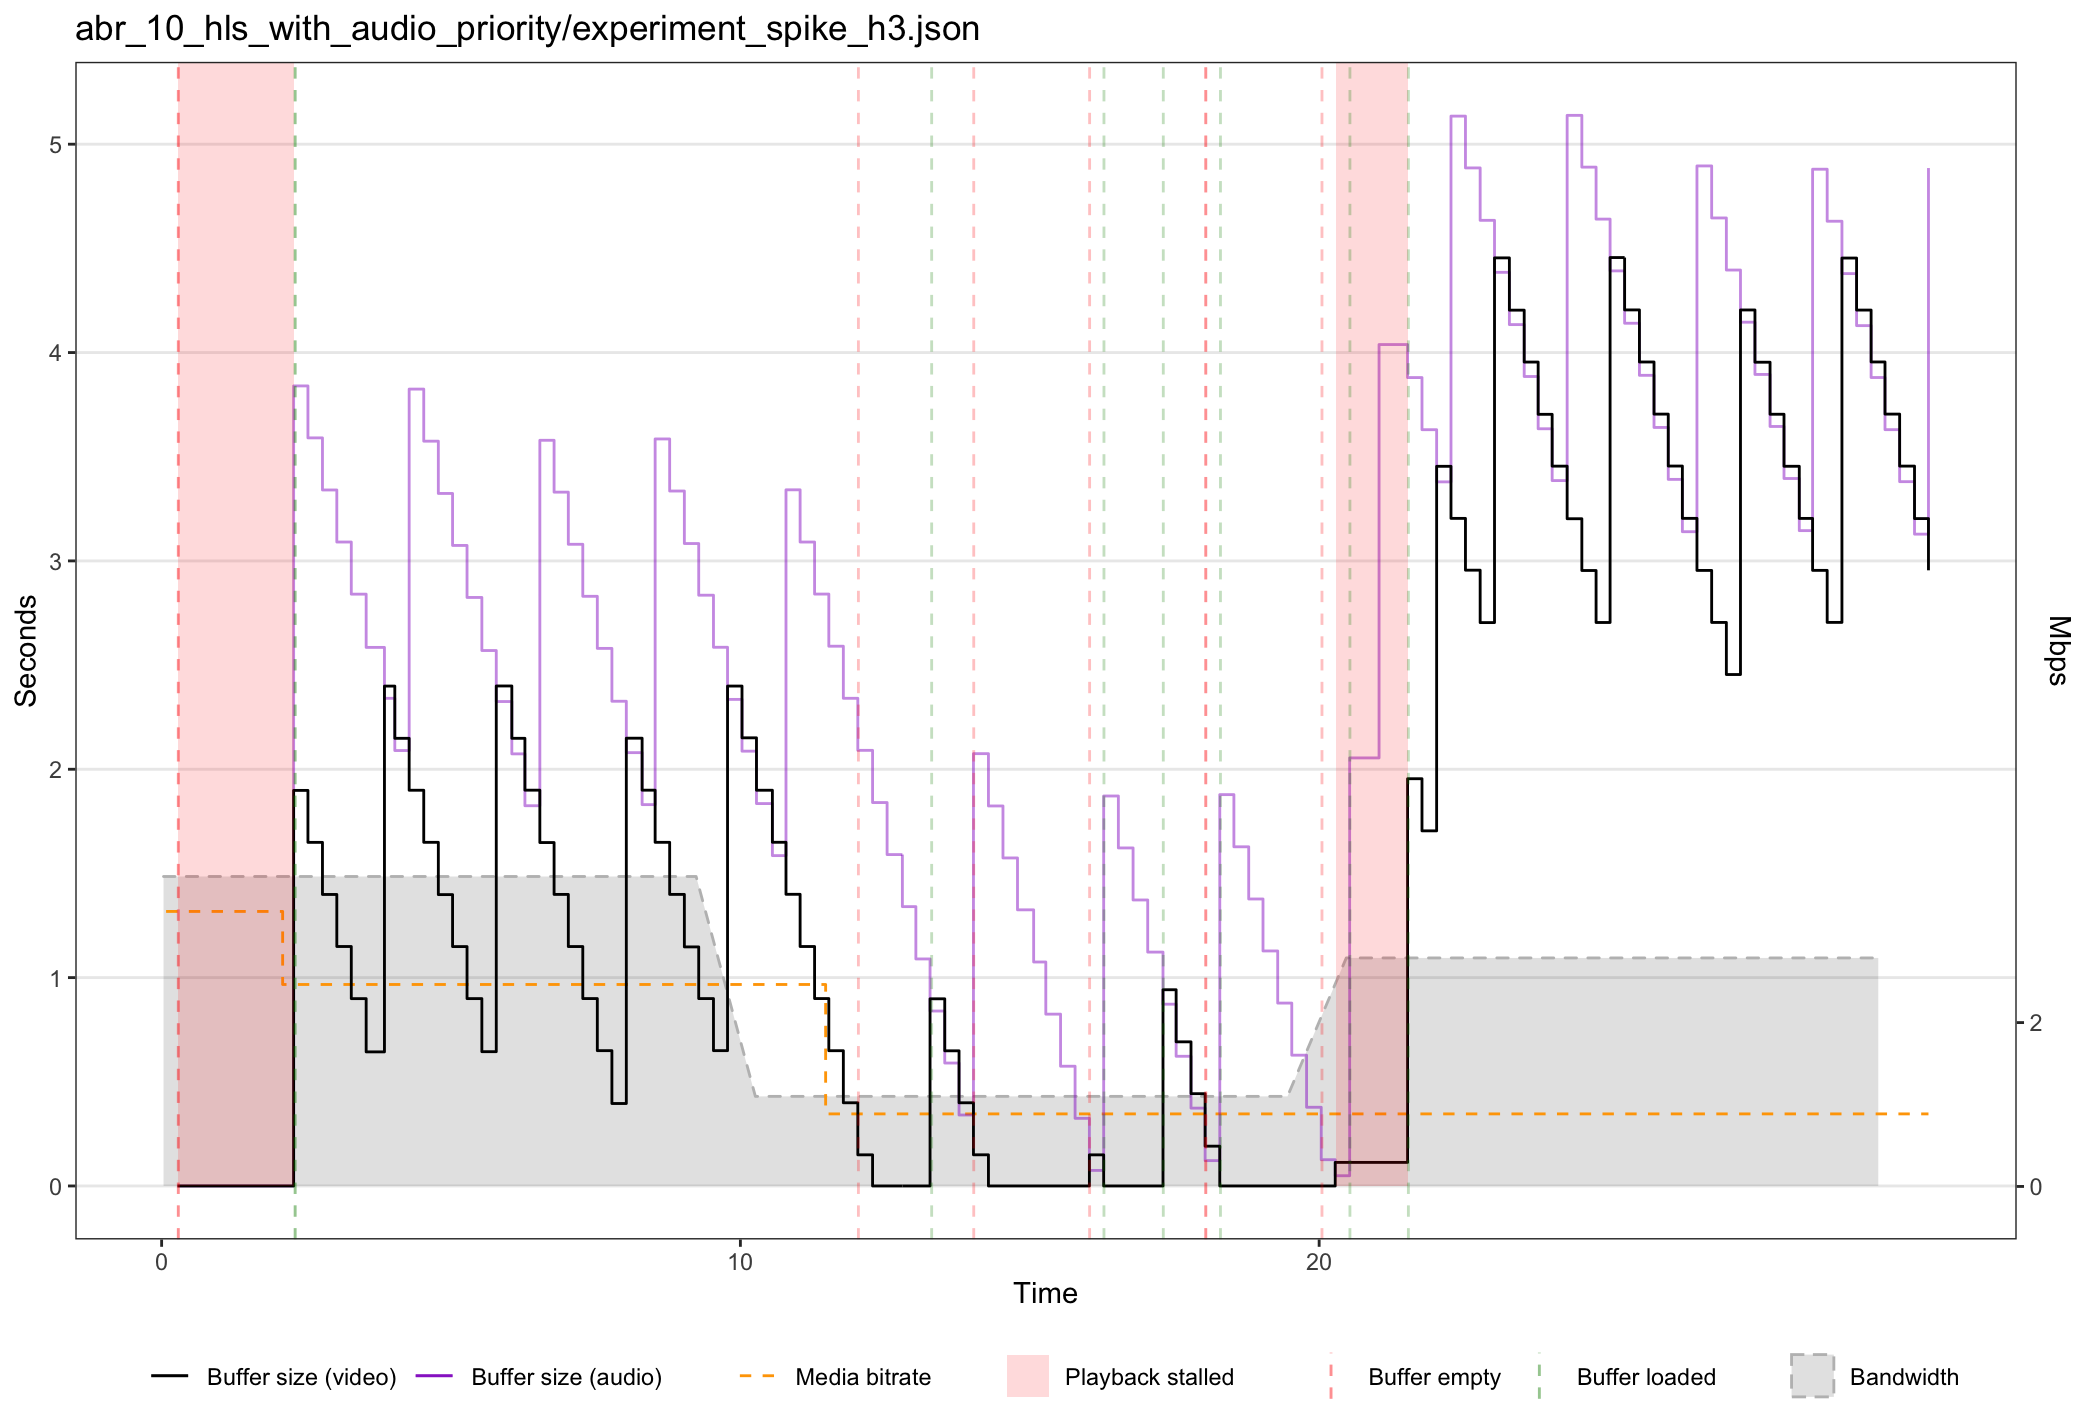
\includegraphics[width=\textwidth]{res/impr_hls_pri.png}
    \caption{Buffer health plot for an HLS experiment with the \texttt{spike} pattern giving priority to the audio.}
    \label{fig:improvements_hls_pri}
\end{figure}

Clearly, when the video buffer is empty the video appears frozen on screen while the buffer recovers, although the audio will keep playing. Unlike the situation where no priority is specified, the live latency of the stream will not increase.

\section{A different live user experience}
\label{sec:improvements/ux}

The behavior that we have shown in the previous section derives from the Chromium implementation of the handling of buffer underflows. This means, for example, that in other browsers when one of the two buffers is empty the playback will immediately stall.

Another limitation is that in Chromium the playback stall is avoided only for three seconds. Ideally, we would like to have more control on how and when this happens, and on all browsers.

The final objective is to build a new user experience that involves less playback stalls. Usually, when a live stream struggles to adapt to network conditions, the user is used to seeing both and audio stop for a while during rebuffering. When this happens, latency tends to grow and the playback will lag behind with respect to the live edge. Consequently, users will receive the action late possibly by even tens of seconds.

However, this kind of live experience is different from what users are used to from other broadcasting systems. For example, digital terrestrial or satellite do not have the concept of buffering: if the video signal is not good enough, video and/or audio are temporarily unavailable while the signal recovers, but no latency is introduced, i.e. viewers always see the live action with a fixed delay independently from the signal quality.

Since we cannot think of completely eliminating rebuffer events, we can instead try to implement a solution that tries to resemble the linear TV experience that viewers are already used to. Although subjective, it would likely result in a better Quality of Experience (QoE).

In practice, this means tackling the following points:

\begin{itemize}
    \item \textbf{Prioritization of requests}: as we have already seen in depth, audio segments and playlists should be prioritized over video.
    \item \textbf{Segment dropping}: when it is too late for a video segment to be useful, we can cancel its download to free bandwidth.
    \item \textbf{Filler/placeholder segments}: when a segment is dropped, we need to provide a placeholder to the source buffer, which should be generated on the client side in the browser.
\end{itemize}

% TODO: related works?

\section{Segment dropping}
\label{sec:improvements/dropping}

In a live stream, when a video segment has no chance of being loaded in time for playback, we can decide that there is no point in continuing the download and instead discard it. In this way, we free bandwidth that can be used to load the next segment.

In HTTP/3, this can be done by aborting the HTTP request, an action that in practice resets the underlying QUIC stream. Resetting a stream means sending a frame of type \texttt{RESET\_STREAM} and immediately closing the stream, also stopping the transmission of the data, if any.

In hls.js, video segments are downloaded sequentially, one at a time. Therefore, we can always look at the current segment and estimate whether the segment will not arrive on time. This is somewhat similar to the \texttt{\_abandonRulesCheck} that we mentioned in \ref{sec:improvements/hlsjs}. That method is called by a JavaScript interval every 100 milliseconds and evaluates whether the current segment is taking too long to load.

In our case, as a first attempt we implemented an even simpler mechanism that simply checks whether we are about to reach the end of the video buffer. We therefore modified the hls.js source code and specifically the \texttt{AbrController}. We added a new periodic timer for a function named \texttt{fillerCheck}, which calculates how much time is left in the buffer.

\begin{minted}[frame=single]{ts}
const bufferInfo = BufferHelper.bufferInfo(
    media,
    media.currentTime,
    config.maxBufferHole
);

const distanceToEndOfBuffer = bufferInfo.len;
const nextFragmentOffset = frag.start - bufferInfo.end;
\end{minted}

The \texttt{distanceToEndOfBuffer} is the buffer length, or the seconds of media data currently contained in the buffer. Obviously, if no data is appended to the buffer it will decrease at every tick of the timer.  The \texttt{nextFragmentOffset} is the time difference between the end of the buffer and the start of the fragment. This is used to understand whether the fragment currently being loaded is the next one. Ideally, the difference should be zero, but timestamps are not always that precise so we use a tolerance threshold.

When the above condition is met and the \texttt{distanceToEndOfBuffer} is less than a threshold, we make the decision to abort the segment load. The threshold was set by default to 200 milliseconds (it must be considered that the tick interval is 100 milliseconds), but it is configurable. One thing that the implementation needs to consider is that the segment loading might be aborted by other rules, for example the \texttt{\_abandonRulesCheck}.

\section{Generating the filler segment}
\label{sec:improvements/filler}

When the segment dropping code makes the decision to discard a video segment, the buffer must be filled with some placeholder data in order not to interrupt playback. We call this segment a \textbf{filler segment}.

To reproduce the Chromium underflow behavior, which consists of showing the last rendered frame on the video canvas while the playback continues with audio, we would need to generate a video segment on the client side by encoding a 2-second video file containing the still picture.

As a first implementation to confirm the feasibility of the solution, we implemented a simpler solution that uses an empty frame with a solid color background. Since H.264 does not necessarily contain timing data, in this way the segment can be generated statically beforehand and even hardcoded in the client code.

However, having the H.264 bitstream is not enough to play the segment. First, the Media Source Extensions API expects muxed data in fMP4, therefore the H.264 data must be correctly inserted in the fMP4 container with the correct timing information.

Moreover, since the filler segment is generated with different encoding parameters than the main stream, there is a discontinuity that the video decoder must be aware of. In fMP4, this signaling of the new parameters is done through initialization segments, that is, segments that contain at least the \texttt{ftyp} and \texttt{moov} boxes. This information is shared by all the segments following the init segment, until a new one is found.

Once both the init segment and the segment data are available, they are appended to the underlying \texttt{SourceBuffer} so that the video segment can be played.

\section{Muxing in the browser}
\label{sec:improvements/muxing}

As mentioned above, once we had the H.264 bitstream for the encoded empty video frame we had to mux it into the fMP4 container to produce the segment. The segment can be composed of only one frame with a duration of 2 seconds, and the correct start timestamp.

The browser APIs do not provide a way to mux or transmux video data, therefore we had to rely on other libraries. An important fact that affects the implementation is that we are dealing with the fragmented MP4 container format and not just MP4. In fact, not all libraries support the fMP4 format.

After investigating possible alternatives, we concluded that there was no complete JavaScript library that implements fMP4 muxing in the browser. In fact, fMP4 muxing is usually performed directly by the libraries that use the MSE API, such as hls.js when transmuxing from MPEG-2 TS to fMP4.

Instead of delving into a manual JavaScript implementation of fMP4 muxing from the raw H.264 bitstream, we decided to experiment with an approach based on \texttt{WebAssembly}.

\texttt{WebAssembly} (WASM) is a low-level binary format that can be used as a build target of many programming languages. It is meant to provide an efficient alternative to JavaScript: a WASM binary file can be embedded and executed in a web page, effectively allowing to execute code written in any supported programming language in the browser at close-to-native performance.

In our case, we took advantage of WASM to execute a Go application to perform the muxing of the video data in the browser. The Go programming language provides out of the box support for building to WASM. For example, to build a \texttt{main.go} file to a WASM binary named \texttt{main.wasm} one would use the command:

\begin{minted}[frame=single]{bash}
GOOS=js GOARCH=wasm go build -o main.wasm main.go
\end{minted}

The Go code built with WASM can then be executed in the browser thanks to a JavaScript utility provided by Go and included with every installation, \texttt{wasm\_exec.js}. In the web page, a simple code snippet such as the following loads the WASM binary file and executes its content.

\begin{minted}[frame=single]{js}
const go = new Go();
WebAssembly.instantiateStreaming(fetch('/main.wasm'), go.importObject)
    .then((result) => {
        go.run(result.instance);
    });
\end{minted}

Within the Go application entrypoint, namely the \texttt{main.go} file, we can directly interact with the Document Object Model (DOM) of the web page. For example, we can access the \texttt{window} object and manipulate the page contents directly. Alternatively, we can expose functions that can then be called by the JavaScript code by setting them as global variables in the \texttt{window} object.

For example, in our case we expose two functions, \texttt{createInit} and \texttt{createSegment}, as shown in Figure \ref{fig:wasm_go_main}. These functions are then called by the TypeScript code when generating the filler segment data.

\begin{figure}[h]
    \centering
    \begin{minted}[frame=single]{go}
//go:build js && wasm
package main
import "syscall/js"

func main() {
	done := make(chan struct{}, 0)
	global := js.Global()
	global.Set("createInit", js.FuncOf(jsCreateInit))
	global.Set("createSegment", js.FuncOf(jsCreateSegment))
	<-done
}
    \end{minted}
    \caption{Caption}
    \label{fig:wasm_go_main}
\end{figure}

Both functions take the H.264 coded data as input, which is then muxed into an fMP4 container. To perform the muxing, we use \texttt{mp4ff}, a library to parse and write MP4 files.\footnote{\url{https://github.com/edgeware/mp4ff}} The input H.264 data must be in the Annex B format with start codes (see Section \ref{sec:bg/compression/codecs/h264}).

For the initialization segment, we must create an fMP4 file containing a \texttt{moov} atom that defines some characteristics of the video tracks. In this case, we only have one video track in the H.264 format, whose decoding information is written in a box that follows the \texttt{avcC} format (see Section \ref{sec:bg/containers/mp4}).

To build the H.264 descriptor, we must first extract two NAL units from the H.264 bitstream, specifically the \textbf{Sequence Parameter Set} (SPS) and the \textbf{Picture Parameter Set} (PPS). These units contain information such as the width and height of the frame and other encoding parameters. Extracting them means parsing the NAL units from the H.264 bitstream and identifying which are the SPS and PPS units, as shown in Figure \ref{fig:wasm_go_sps}.

\begin{figure}[h]
    \centering
    \begin{minted}[frame=single]{go}
func ExtractSpsPps(bitstream []byte) ([]byte, []byte) {
	nalus := avc.ExtractNalusFromByteStream(bitstream)
	var sps []byte
	var pps []byte
	for _, nalu := range nalus {
		switch avc.GetNaluType(nalu[0]) {
		case avc.NALU_SPS:
			sps = nalu
		case avc.NALU_PPS:
			pps = nalu
		}
	}
	return sps, pps
}
    \end{minted}
    \caption{Caption}
    \label{fig:wasm_go_sps}
\end{figure}

The init segment can then be built by adding the \texttt{moov} boxes, which contains a single \texttt{trak} with the \texttt{avcC} information. In this step, we also need to assign a time scale to the video track. The time scale represents the number of time units per second, and is then used as a basis for assigning a timestamp to the specific video frame. For example, if we set the time scale to 12800, a typical value, it means that in a 25 fps video file each frame will have a timestamp that is a multiple of 512.

The \texttt{createSegment} function is instead used to create the actual media segment, or fMP4 fragment. The inputs of this function are not only the H.264 bitstream as for the \texttt{initSegment} function, but also the start timestamp of the segment and its duration, both in seconds.

In the actual implementation, we must create another fragmented MP4 file instance and only add one fragment to it. Since the Annex B packetization format is incompatible with MP4, we must first convert the byte stream to NALU samples. The library \texttt{mp4ff} provides us with an helper function to do this.

We then need to add the video frames to the segment. In our case, we have a single frame which we will put in an MP4 sample with a duration of 2 seconds. Note that the timestamp and duration need to be expressed in terms of the time scale, as mentioned before. Figure \ref{fig:wasm_go_fragment} shows a simplified piece of code that creates the sample and adds it to the fragment.

\begin{figure}[h]
    \centering
    \begin{minted}[frame=single]{go}
bitstream = avc.ConvertByteStreamToNaluSample(bitstream)

sample := mp4.FullSample{
	Sample: mp4.Sample{
		Flags:                 mp4.SyncSampleFlags,
		Dur:                   uint32(TimeScale * duration),
		Size:                  uint32(len(bitstream)),
		CompositionTimeOffset: 0,
	},
	DecodeTime: uint64(TimeScale * timestamp),
	Data:       bitstream,
}

frag.AddFullSample(sample)
    \end{minted}
    \caption{Caption}
    \label{fig:wasm_go_fragment}
\end{figure}






% TODO: hls.js internals

% TODO: webcodecs


